\documentclass{llncs}

\usepackage{graphicx}
\usepackage{shortcuts}
\usepackage{xspace}
\usepackage{code}
\usepackage{cite}
\usepackage{url}
\usepackage{listings}
\usepackage{boxedminipage}
\usepackage{times}
\usepackage{multirow}
\usepackage{algorithmic}
\usepackage{algorithm}

%\usepackage[text={6.5in,9in},centering]{geometry}

\pagestyle{plain}

\begin{document}

\title{UserCSP:User Specified Content Security Policy}

\author{Kailas Patil\inst{1} \and Tanvi Vyas\inst{2}}
\institute{National University of Singapore \\ \email{patilkr@comp.nus.edu.sg} \and Mozilla \\\email{tanvi@mozilla.com} }


 

\maketitle

\begin{abstract}

According to OWASP top vulnerability list, cross-site scripting (XSS)
is among the top five web application vulnerabilities. It allows
attackers to inject malicious code or resources from attacker domains
into the DOM of a vulnerable web page. Browsers are not able to
distinguish between legitimate and malicious content. Therefore,
Content Security Policy (CSP) is a mechanism that enables the browser
to identify potentially malicious injected content in web pages.


By-default CSP doesn't allow inline scripts and eval, which are used
by almost all website. To use CSP, websites are required to change
their code or allow these potential attack vectors, and hence mitigate
the effectiveness of CSP. The code change requirement is hindering the
adaptation of CSP by web applications (websites). However, there are
savvy users who prefer security over usability. In addition, website
developers need a tool to test different CSP rules for their website
that secure their users and also achieve usability. To address these
issues we propose \codename and prototype our approach in a Firefox
extension using the JetPack framework. \codename allows savvy users to
specify CSP rules to particular websites or to specify general CSP
rules that are enforced on each and every website a user
visits. Moreover, it allows website developers to try out different
CSP rules and iterate to achieve the best suited CSP policy for their
website.

\end{abstract} 


{\bf Keywords:} content security policy, web security, security policy, content restrictions 


\section{Introduction}
\label{sec:background}

The web browsers security model is rooted in the sameorigin policy
(SOP) ~\cite{sop}, which isolates resources of one origin from
others. However, attackers can subvert the SOP by injecting malicious
contents into a vulnerable website; this is known as Cross-site
scripting (XSS) attacks~\cite{xss}. Cross-site Scripting (XSS) attacks
in web applications are considered a major threat. XSS allows an
attacker to conduct a wide range of potential attacks, such as session
hijacking, stealing sensitive data and passwords, creation of
self-propagating JavaScript worms, etc. To mitigate XSS attacks,
Content Security Policy (CSP)~\cite{csp} provide website
administrators with a way to enforce content restrictions at the
client side.

Content Security Policy is a declarative policy that restricts what
content can be loaded on a web page. Its primary purpose is to
mitigate Cross-Site Scripting vulnerabilities.  The core issue
exploited by Cross-Site Scripting (XSS) attacks is that web browsers
lack the knowledge to distinguish between content that's intended to
be part of a web application, and content that's been maliciously
injected into a web application. To address this problem, CSP defines
the {\tt Content-Security-Policy} HTTP header that allows web application
developers to create a whitelist of trusted content sources, and
instruct the client browsers to only execute or render resources from
those sources. However, it is often difficult for developers to write
a comprehensive Content Security Policy for their website. They may
worry about their page breaking because unanticipated but necessary
content is blocked. They may not be able to easily change the headers
their site is sending when these situations occur, which makes it
difficult for them to try different policies until they find one that
is the most restrictive for their page without breaking site
functionality.

UserCSP changes this! A developer or user can now view the current
policy set by their site and add their own policy.  They can choose to
apply their custom policy on the site, or even combine their policy
with the website’s existing policy.  When combining policies, they
have an option to choose from the strictest subset of the two, or the
most lax subset.  They can locally test their site with the custom
policy applied and tweak the policy until they have one that works.

UserCSP also allows automatic inference of a Content Security Policy
for a website. Automatically inferred policies for a website help web
developers figure out what CSP rules to set for their site by giving
them the strictest possible policy they could apply without breaking
the current page.  To infer the CSP policy for a website, UserCSP
analyzes the content on the current web page and recommends a CSP
based on the content types and content sources. UserCSP provides this
inferred policy to developers in the proper syntax for the CSP header,
so all a developer needs to do is start serving this policy for their
site via the CSP header. [Moreover, it allows users to enforce
  inferred policy on the website.-REMOVE] Furthermore, UserCSP allows
savvy users to voluntarily specify their own Content Security Policy
for websites that may not have implemented CSP.

In summary, this paper makes the following contributions:

\begin {itemize}

\item We present an automated approach, UserCSP, for writing a Content
  Security Policy for a website.

\item UserCSP allows savvy users to voluntarily specify their own
  Content Security Policy for websites that may not have implemented
  CSP.

\item We implemented a prototype of our approach in a Firefox
  extension.

\end{itemize}

\section{Background}
\label{sec:back}
Content Security Policy (CSP) helps to detect and mitigate attacks
such as Cross-site scripting(XSS) and Clickjacking.
 
\subsection{Cross-site Scripting (XSS)}
Cross-site Scripting (XSS) or script injection is well known
vulnerability in web applications. According to Web Hacking Incident
Database (WHID) 2010 semiannual report, XSS was in the top in the list
of application security risks~\cite{WHID-2010report}.  In XSS attack
malicious script is injected into an otherwise trusted web page
violating integrity of infected web application and causing an
unexpected behavior such as stealing sensitive information or
modifying server side state of a user. When a user visits a web page
of trusted site that contains malicious injected script, the injected
script is executed in user's browser with the principle of trusted
site. Therefore, injected scripts have full control over the session and
thus can send arbitrary requests with valid session and security
tokens.

\begin{figure}[h!]
\begin{center}
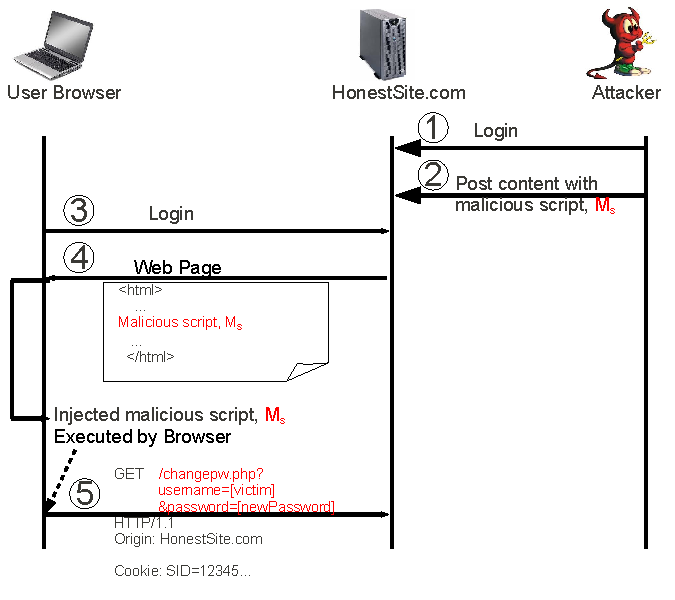
\includegraphics[width=0.7\textwidth]{xss-example}
\end{center}
\caption{Illustration of Cross-Site Scripting}
\label{fig:xssIll}
\end{figure}

\paragraph{\bf An Example of XSS Attack.}
If user visits a web page of vulnerable trusted web site, say {\em
  HonestSite.com} in which attacker has injected inline malicious
script, say $M_{s}$. Malicious script, $M_s$, is executed in the
context of web site and can send state modifying request to {\em
  HonestSite.com}

As shown in Figure~\ref{fig:xssIll}, attacker first login to a web
site, {\em HonestSite.com} (Step 1). On the vulnerable web page of the
web site, attacker submits malicious script, $M_s$ (Step 2). When user
login to the web site (Step 3), and visits the vulnerable web page
(Step 4), injected malicious script, $M_s$ is executed in the context
of web site. When injected script executed in the context of web site
it will compromise the integrity of web site by sending malicious
request to modify user state of the user on the web site (Step
5). Request is generated by injected script running with the principle
of web site, therefore web site processes the malicious request
generated by injected script. Moreover, injected script when executed
with the principle of web site it can also steal sensitive information
such as username/password, cookies, etc and send them to attacker's
domain.

\paragraph{\bf Mitigation of Cross-site Scripting(XSS).}
Content security policy allows website administrators to eliminate
their XSS attack surface. To achieve this goal, CSP allows website
administrators specify which domains the browser should treat as valid
sources of script. Moreover, the web browser will only execute script
in source files from the white-listed domains and will disregard
everything else, including inline scripts.

\subsection{Clickjacking}
In Clickjacking attacks~\cite{nex08,sectheory08}, attackers exploit
the layout feature introduced by iFrames. Specifically, they load a
victim web page into an iFrame on the top and make it
transparent. Then they load a deceptive page in another iFrame at the
bottom layer to attract users to click.

\paragraph{\bf An Example of Clickjacking.}

\begin{figure}[!ht]
\begin{center}
\fbox{\parbox{\columnwidth}{
    {\tt
%%\begin{verbatim}
\textless -- Page from www.Websitename.com --\textgreater

<html>

...

<iframe id="victim" src="http://example.com" scrolling="no" 

\hspace*{1.0cm}width="600px" height="600px" style="opacity:0; 

\hspace*{1.0cm}position:absolute; left:10px; top:10px;">

</iframe>

...

<div style = "position:absolute; top:Ypx;left:Xpx;">

\hspace*{1.0cm}<a href= "http://example.com">Click Here</a>

</div>

...

</html>
%%\end{verbatim}
}
}}
\end{center}
  %%\vspace{-0.3in}
\caption{\small Clickjacking using transparent iFrame and overlay objects.}
\label{fig:clickGuardoverlayobject}
\end{figure}


\begin{figure}[!ht]
\begin{center}
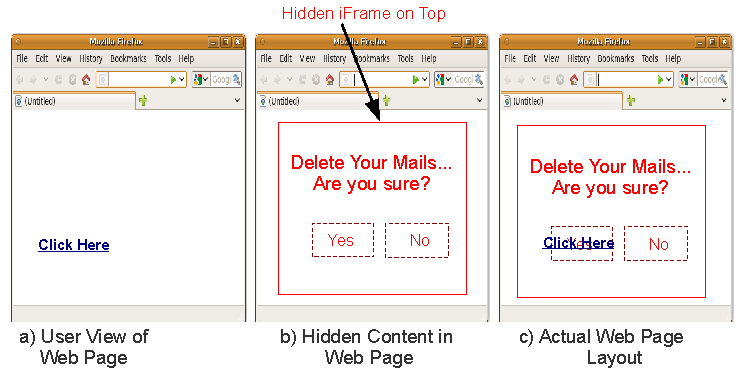
\includegraphics{overlayExa}
\end{center}
%%  \vspace{-0.3in}
\caption{\small Illustration of Clickjacking using transparent iFrame
  and overlay objects}
\label{fig:clickGuardoverlayobjectIll}
\end{figure}

Figure~\ref{fig:clickGuardoverlayobject} shows an example of a
Clickjacking attack. The front page of {\tt http://example.com} is
loaded inside a transparent iFrame (zero opacity value to make it
transparent). To lure users to click at a particular location of the
page loaded inside the transparent iFrame, the attacker creates a link
in the visible bottom layer, which is located exactly at the same
position where the attacker wants users to click in the top layer. As
shown in Figure~\ref{fig:clickGuardoverlayobject}, the attacker
specifies the location of a link by setting its X and Y
coordinates. When users try to click on the link, they actually click
on the transparent layer of the iFrame loaded with the page from {\tt
  example.com}. An illustration of such a Clickjacking attack is
presented in Figure~\ref{fig:clickGuardoverlayobjectIll}.


\paragraph{\bf Mitigation of Clickjacking.}
Content Security Policy enables a protected website {\tt S} to specify
which websites can embed {\tt S}. That is, a protected website {\tt S}
can decide what other websites it trusts to embed it.

\section{UserCSP Design}
\label{sec:design}

The goal of our approach, UserCSP, is to help web site
administrators and website users to write comprehensive
CSP rules for the website.

\begin{figure}[!ht]
\center
  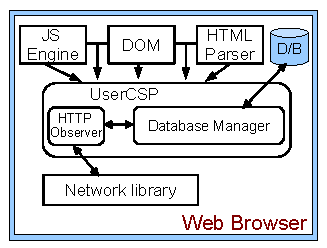
\includegraphics{userCSP_Arch}
\caption{UserCSP Architecture}
\label{fig:userCSP-Arch}
\end{figure}

Figure~\ref{fig:userCSP-Arch} illustrates the architecture of
UserCSP. To enforce user specified Content Security Policy as well as
to infer CSP policy for a website, UserCSP monitors web browsers
internal events including HTML parsing, HTTP requests, XHR, etc., and
analyzes the type of content loaded by a web page and source of that
content. Database manager component of the UserCSP is responsible for
storing user specified CSP rules for websites into local database and
retrieves the corresponding CSP rules for the website when user loads
the website.

When users visits a website, UserCSP performs one of
the following actions:


\begin{itemize}

\item If website has defined CSP, but the user hasn��t specified a CSP
  policy for that website, then UserCSP doesn��t interfere with the
  website defined CSP rules.  However, it allows the user the option
  to amend the website's CSP.

\item If a user has specified CSP rules for a website, but the website
  administrators hasn��t defined a CSP for their website, then the user
  specified CSP policy will be enforced by the UserCSP.
 
\item If a user specified CSP exists as well as a website defined CSP,
  then users have a choice either to apply their own policy or adopt
  the website defined policy. Moreover, users can also select a strict
  or loose set of CSP rules by combining their own policy with the
  website defined policy. For example, if a website sets ��script-src
  www.example.com;�� and user specifies ��script-src www.example.com
  www.abc.com;�� then the strict policy would be ��script-src
  www.example.com;�� whereas the loose policy would be ��script-src
  www.example.com www.abc.com;��.

\item If neither user nor website administrators specifiy a CSP for a
  website then UserCSP doesn��t interfere with the content loading on
  the website.

\item To allow automatic inference of a CSP for websites, UserCSP
  monitors content loaded by web pages and recommends CSP rules based
  on the types of content and sources of that content. It also
  monitors the resources dynamically added to the web page by
  JavaScript.

\end{itemize}

\section {Implementation of UserCSP}
\label{sec:imp}

\begin{figure}[!ht]
\begin{center}
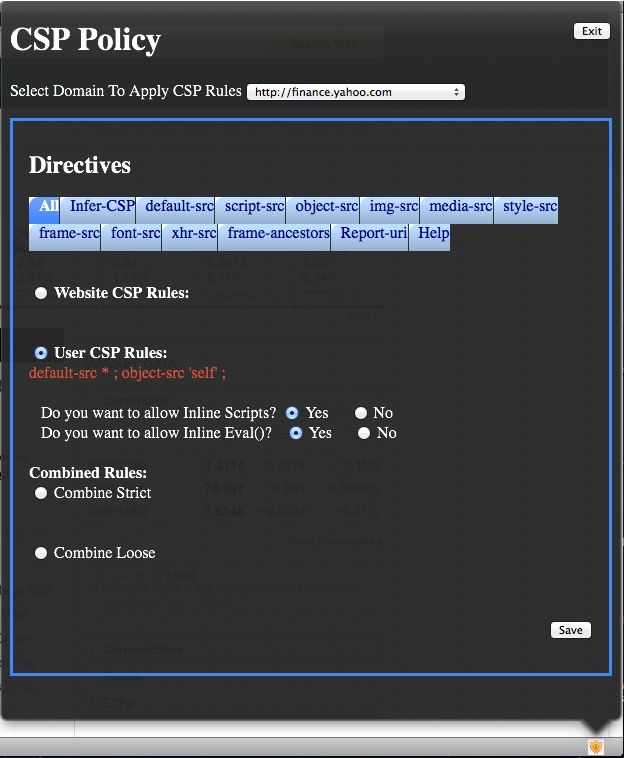
\includegraphics[width=0.7\textwidth]{UserCSP-ui}
\end{center}
\caption{UserCSP UI}
\label{fig:userCSP-ui}
\end{figure}

We implemented UserCSP \footnote[1]{UserCSP Source Code:
  https://github.com/patilkr/userCSP} in Firefox extension using the
Jetpack SDK v1.9~\cite{JetPack-SDK}. UserCSP intercepted various
events, including the {\it READY}, {\it ACTIVATE}, and {\it CLOSE} events on
tab. The READY event is used to retrieve a list of open websites in a
user's Firefox web browser. The ACTIVATE event is used to select the
currently active domain in the web browser.  The CLOSE event is used
to remove the domain name from the UI if a user closes the
tab. UserCSP uses a sqlite database to store user specified CSP rules
for websites.

The {\it http-on-examine-response} observer notification is used to
intercept the HTTP response. In the intercepted response, the domain
that initiated the request is checked against the sqlite local
database to determine whether user defined rules were set. If there
are no rules associated with the website, the response is processed
without any change.  However, if user defined CSP rules exist, the
{\tt Content- Security-Policy} header is added to the response with
the rules specified by the user. If user has opted to enforce their
own rules then UserCSP replaces the existing {\tt Content-Security-Policy} header if it is already set by the website.

Figure~\ref{fig:userCSP-ui} shows graphical user interface of UserCSP
add-on we developed as an extension to Mozilla Firefox. The userCSP
add-on UI contains drop-down list for domain selection. The domain
selection list contains the websites that the user has opened in the
browser. For example, \url{http://finance.yahoo.com/} is shown in the
Figure. In addition to this, domain selection drop-down list also
contains an entry {\tt * (Every Website)}. The {\tt * (Every Website)}
option is used to allow users to specify general rules for all
websites the users visits that do not have a website or user CSP
policy set. If a user has set a policy for website and also set a
policy for {\tt * (Every Website)}, then the user policy set for the
website takes precedence over the {\tt * (Every Website)}. If a
website has set a CSP policy in their header and the user has set a
policy for {\tt * (Every Website)}, then the policy set by the website
takes precedence over the {\tt * (Every Website)}.

Moreover, for each domain there are total 14 tabs provided to user as
shown in the Figure~\ref{fig:userCSP-ui} namely, {\tt All, Infer-CSP,
  default-src, script-src, object-src, image-src, media-src,
  style-src, frame-src, font-src, xhr-src, frame-ancestors,
  report-uri, Help}. Except for the 'All', 'Infer Policy', and 'Help'
tab, the other tabs are CSP directives used in Firefox. They are used
to allow a user to specify a CSP rule for that CSP directive. The
'All' tab is used to display the complete website defined CSP policy,
as well as complete user defined CSP policy. It also allows users to
calculate the Strictest Policy and Loosest Policy from the user
defined CSP and the website defined CSP. Moreover, it also allows user
to select a policy for a website from the four possible values -
Website CSP rules, User CSP rules, Combine Strict Rules or Combine
Loose Rules. By-default website CSP rules are selected. In addition to
this, when the User CSP rules are selected, the 'All' tab also allows
users to enable or disable inline scripts and inline evals.

\paragraph{\bf Combine Strict CSP:} If both website and user defined CSP rules for a website are available then this feature allow users to apply the strictest subset CSP policy which is calculated from the website defined CSP and the user defined CSP. For example, when you strictly combine website specified policy {\tt img-src 'self'} with user specified policy {\tt img-src '*'}, the combined policy {\tt img-src 'self'} is set.

\paragraph{\bf Combine Loose CSP:} If both website and user defined CSP rules for a website are available then this feature allow users to apply the loosest subset CSP policy which is calculated from the website defined CSP and the user defined CSP. For example, when you loosely combine website specified policy {\tt img-src 'self'} with user specified policy {\tt img-src "*"}, the combined policy {\tt img-src '*'} is set.

\tanvi{ [Kailas - unless the user has selected to apply website rules
    instead of their own rules.  Maybe add something about that]}


\section{Evaluation}
\label{sec:eval}

We implemented our approach in Firefox v14.0 using JetPack SDK
v1.9. We used Alexa Top 10 Sites \footnote[2]{Alexa top 10 sites used
  for evaluation were: facebook.com, google.co.in, youtube.com,
  yahoo.com, baidu.com, wikipedia.org, live.com, twitter.com, qq.com,
  and amazon.com} to test our approach against user defined CSP
policies as well as automatically inferred CSP policies. Automatically
inferred CSP policies don��t break websites whereas manually defined
CSP policies required several rounds of refinement and web page source
code inspection to record content sources. The reason for that is
initially we set CSP rules for a website to load resources from its
own domain only, but websites were loading content from CDN��s or
sub-domains. Appendix~\ref{appendix} shows examples of inferred CSP
policies.


\section{Related Work}
\label{sec:relwork}
Content Security Policy(CSP)~\cite{csp} provides content restriction
enforcement that allows web sites to specify which sites are trusted
and then rely on the user’s browser to forbid loading resources from
untrusted sites or from the sites not in the list specified by the web
application.  We extended CSP mechanism to allow users to specify CSP
policy for a web site, and then enforce it. 

BEAP~\cite{beap} mitigates the CSRF attack at client side. It infers
whether a request reflects user's intention using the heuristics
derived from analyzing real-world web applications. If a sensitive
request does not reflects users' intention, BEAP strips authentication
token from it. Whereas CSP blocks all requests except for those that
the web site has explicitly granted.  

Browser-enforce Embedded Policies (BEEP)~\cite{beep} aims to allow web
applications to specify which scripts can run on its web site. As
compared to our approach, BEEP is limited to restricting scripts that
can run on a web site, whereas other contents such as images, frames,
style sheets, etc are not restricted.

%%\input{discussion}
\section{Conclusion}
\label{sec:conclu}

In complex web application attackers find various ways to inject
malicious content in a website. Content Security Policy (CSP) provides
content restrictions mechanism to allow web site administrators to
control at client side, what types of content can be loaded and from
what sources it can be loaded. It also provides ability to web
browsers to distinguish web site intended contents and injected
content. In this work, we present an approach, \codename, that helps
web administrators as well as users to write compressive CSP policy
for a website. It also automatically infer CSP policy for a
website. Our prototype was implemented in the Firefox extension using
the JetPack SDK.


%% \section*{Acknowledgments}
%% We thank Sid Stamm for his help on the implementation of UserCSP.  We
%% thank the anonymous reviewers for their valuable comments. This work
%% is in part supported by the NUS Young Investigator Award
%% R-252-000-378-101.

\bibliographystyle{plain}
\bibliography{paper}

\newpage
\section {Appendix: Examples of inferred CSP policy by \Codename}
\label{appendix}

CSP policies that were automatically inferred by \codename for
\url{www.facebook.com} and \url{in.yahoo.com} are given below:

\paragraph{\bf Inferred CSP policy for www.facebook.com}
Figure~\ref{fig:facebookCSP} shows an inferred CSP policy by \codename
for \url{www.facebook.com}.

\begin{figure}[h!]
\small
\begin{verbatim}
default-src 'self'; 
script-src http://static.ak.fbcdn.net; 
img-src http://photos-g.ak.fbcdn.net
        http://photos-c.ak.fbcdn.net 
        http://photos-a.ak.fbcdn.net 
        http://photos-b.ak.fbcdn.net 
        http://secure-us.imrworldwide.com 
        http://static.ak.fbcdn.net 
        http://profile.ak.fbcdn.net; 
style-src  http://static.ak.fbcdn.net;  
\end{verbatim}
\caption{Inferred CSP for www.facebook.com}
\label{fig:facebookCSP}
\end{figure}



\paragraph{\bf Inferred CSP for in.yahoo.com/?p=us}
Figure~\ref{fig:yahooCSP} shows an inferred CSP policy by \codename
for \url{in.yahoo.com}.

\begin{figure}[h!]
\small
\begin{verbatim}
default-src 'self'; 
script-src http://bs.serving-sys.com 
           http://l.yimg.com 
           http://mi.adinterax.com; 
object-src http://mi.adinterax.com ;
img-src http://l.yimg.com 
        http://l1.yimg.com 
        http://d.yimg.com 
        http://ads.yimg.com 
        http://ad.yieldmanager.com 
        http://ds.serving-sys.com 
        http://b.scorecardresearch.com 
        http://row.bc.yahoo.com; 
style-src http://l.yimg.com; 
frame-src http://ads.yimg.com 
          http://ad.yieldmanager.com; 
\end{verbatim}
\caption{Inferred CSP for in.yahoo.com}
\label{fig:yahooCSP}
\end{figure}




\end{document}
